% Diagram comparing LaTeX with Word.
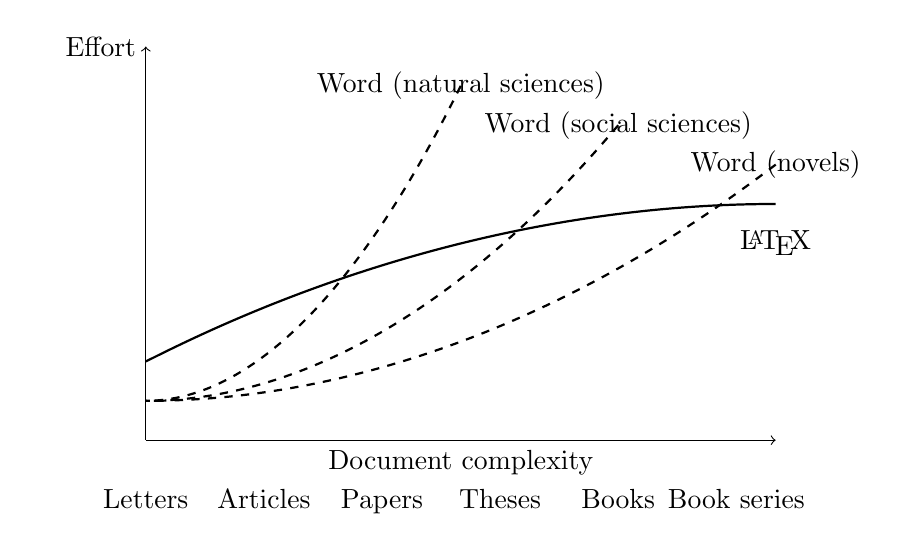
\begin{tikzpicture}

% horizontal axis
\draw[->] (0,0) -- (8,0) node[anchor=north,midway] {Document complexity};
\draw[->] (0,0) -- (0,5) node[anchor=east] {Effort};

% labels
\draw	(0,-0.5) node[anchor=north] {Letters}
		(1.5,-0.5) node[anchor=north] {Articles}
		(3,-0.5) node[anchor=north] {Papers}
		(4.5,-0.5) node[anchor=north] {Theses}
		(6,-0.5) node[anchor=north] {Books}
		(7.5,-0.5) node[anchor=north] {Book series};

\draw (8,3.5) node {Word (novels)};
\draw (6,4) node {Word (social sciences)};
\draw (4,4.5) node {Word (natural sciences)};
\draw (8,2.5) node {\LaTeX{}};

% Psis
\draw[thick,dashed] (8,3.5) parabola[bend at end] (0,0.5);
\draw[thick,dashed] (6,4) parabola[bend at end] (0,0.5);
\draw[thick,dashed] (4,4.5) parabola[bend at end] (0,0.5);
\draw[thick] (0,1) parabola[bend at end] (8,3);
\useasboundingbox (-1.5,-0.2);
\end{tikzpicture}